\documentclass[11pt]{article}
\usepackage{amsgen,amsmath,amstext,amsbsy,amsopn,amssymb}
%\usepackage[dvips]{graphicx,color}
\usepackage{graphicx,color}
\usepackage{graphicx,color,bm}
\usepackage{epsfig}
\usepackage{enumerate}
\usepackage{float}

%\setlength{\oddsidemargin}{0.1 in} \setlength{\evensidemargin}{-0.1
%in} \setlength{\topmargin}{-0.6 in} \setlength{\textwidth}{6.5 in}
%\setlength{\textheight}{8.5 in} \setlength{\headsep}{0.75 in}
%\setlength{\parindent}{0 in} \setlength{\parskip}{0.1 in}

\textwidth 6.3in \textheight 8.8in \topmargin -0.5truein
\oddsidemargin .15truein
\parskip .1in
\renewcommand{\baselinestretch}{1.53}  % double spaced


\newcommand{\homework}[9]{
	\pagestyle{myheadings}
	\thispagestyle{plain}
	\newpage
	\setcounter{page}{1}
	\noindent
	\begin{center}
		\framebox{
			\vbox{\vspace{2mm}
				\hbox to 6.28in { {\bf Math531:~Regression - I  \hfill} }
				\vspace{6mm}
				\hbox to 6.28in { {\Large \hfill #1 (#2)  \hfill} }
				\vspace{6mm}
				\hbox to 6.28in { {\it Instructor: #3 \hfill} }
				\hbox to 6.28in { {\it Office hours: #4  \hfill #6}}
				\vspace{2mm}}
		}
	\end{center}
	\markboth{#1}{#1}
	\vspace*{4mm}
}

% ----------------------- MATH -------------------------
\def\av{\boldsymbol a}
\def\bv{\boldsymbol b}
\def\cv{\boldsymbol c}
\def\dv{\boldsymbol d}
\def\ev{\boldsymbol e}
\def\fv{\boldsymbol f}
\def\gv{\boldsymbol g}
\def\hv{\boldsymbol h}
\def\iv{\boldsymbol i}
\def\gv{\boldsymbol j}
\def\kv{\boldsymbol k}
\def\lv{\boldsymbol l}
\def\mv{\boldsymbol m}
\def\nv{\boldsymbol n}
\def\ov{\boldsymbol o}
\def\pv{\boldsymbol p}
\def\qv{\boldsymbol q}
\def\rv{\boldsymbol r}
\def\sv{\boldsymbol s}
\def\tv{\boldsymbol t}
\def\uv{\boldsymbol u}
\def\vv{\boldsymbol v}
\def\wv{\boldsymbol w}
\def\xv{\boldsymbol x}
\def\yv{\boldsymbol y}
\def\zv{\boldsymbol z}
\def\Av{\boldsymbol A}
\def\Bv{\boldsymbol B}
\def\Cv{\boldsymbol C}
\def\Dv{\boldsymbol D}
\def\Ev{\boldsymbol E}
\def\Fv{\boldsymbol F}
\def\Gv{\boldsymbol G}
\def\Hv{\boldsymbol H}
\def\Iv{\boldsymbol I}
\def\Gv{\boldsymbol J}
\def\Kv{\boldsymbol K}
\def\Lv{\boldsymbol L}
\def\Mv{\boldsymbol M}
\def\Nv{\boldsymbol N}
\def\Ov{\boldsymbol O}
\def\Pv{\boldsymbol P}
\def\Qv{\boldsymbol Q}
\def\Rv{\boldsymbol R}
\def\Sv{\boldsymbol S}
\def\Tv{\boldsymbol T}
\def\Uv{\boldsymbol U}
\def\Vv{\boldsymbol V}
\def\Wv{\boldsymbol W}
\def\Xv{\boldsymbol X}
\def\Yv{\boldsymbol Y}
\def\Zv{\boldsymbol Z}
\def\Abf{\mathbf A}
\def\Bbf{\mathbf B}
\def\Cbf{\mathbf C}
\def\Dbf{\mathbf D}
\def\Ebf{\mathbf E}
\def\Fbf{\mathbf F}
\def\Gbf{\mathbf G}
\def\Hbf{\mathbf H}
\def\Ibf{\mathbf I}
\def\Gbf{\mathbf J}
\def\Kbf{\mathbf K}
\def\Lbf{\mathbf L}
\def\Mbf{\mathbf M}
\def\Nbf{\mathbf N}
\def\Obf{\mathbf O}
\def\Pbf{\mathbf P}
\def\Qbf{\mathbf Q}
\def\Rbf{\mathbf R}
\def\Sbf{\mathbf S}
\def\Tbf{\mathbf T}
\def\Ubf{\mathbf U}
\def\Vbf{\mathbf V}
\def\Wbf{\mathbf W}
\def\Xbf{\mathbf X}
\def\Ybf{\mathbf Y}
\def\Jbf{\mathbf J}
\def\Zbf{\mathbf Z}
\def\Am{\mathrm A}
\def\Bm{\mathrm B}
\def\Cm{\mathrm C}
\def\Dm{\mathrm D}
\def\Em{\mathrm E}
\def\Fm{\mathrm F}
\def\Gm{\mathrm G}
\def\Hm{\mathrm H}
\def\Im{\mathrm I}
\def\Gm{\mathrm J}
\def\Km{\mathrm K}
\def\Lm{\mathrm L}
\def\Mm{\mathrm M}
\def\Nm{\mathrm N}
\def\Om{\mathrm O}
\def\Pm{\mathrm P}
\def\Qm{\mathrm Q}
\def\Rm{\mathrm R}
\def\Sm{\mathrm S}
\def\Tm{\mathrm T}
\def\Um{\mathrm U}
\def\mv{\mathrm V}
\def\Wm{\mathrm W}
\def\Xm{\mathrm X}
\def\Ym{\mathrm Y}
\def\Zm{\mathrm Z}
\newcommand{\Ac}{\mathcal{A}}
\newcommand{\Bc}{\mathcal{B}}
\newcommand{\Cc}{\mathcal{C}}
\newcommand{\Dc}{\mathcal{D}}
\newcommand{\Ec}{\mathcal{E}}
\newcommand{\Fc}{\mathcal{F}}
\newcommand{\Gc}{\mathcal{G}}
\newcommand{\Hc}{\mathcal{H}}
\newcommand{\Ic}{\mathcal{I}}
\newcommand{\Jc}{\mathcal{J}}
\newcommand{\Kc}{\mathcal{K}}
\newcommand{\Lc}{\mathcal{L}}
\newcommand{\Mc}{\mathcal{M}}
\newcommand{\Nc}{\mathcal{N}}
\newcommand{\Oc}{\mathcal{O}}
\newcommand{\Pc}{\mathcal{P}}
\newcommand{\Qc}{\mathcal{Q}}
\newcommand{\Rc}{\mathcal{R}}
\newcommand{\Sc}{\mathcal{S}}
\newcommand{\Tc}{\mathcal{T}}
\newcommand{\Uc}{\mathcal{U}}
\newcommand{\Vc}{\mathcal{V}}
\newcommand{\Wc}{\mathcal{W}}
\newcommand{\Xc}{\mathcal{X}}
\newcommand{\Yc}{\mathcal{Y}}
\newcommand{\Zc}{\mathcal{Z}}
\newcommand{\alphav}{\mbox{\boldmath{$\alpha$}}}
\newcommand{\betav}{\mbox{\boldmath{$\beta$}}}
\newcommand{\gammav}{\mbox{\boldmath{$\gamma$}}}
\newcommand{\deltav}{\mbox{\boldmath{$\delta$}}}
\newcommand{\epsilonv}{\mbox{\boldmath{$\epsilon$}}}
\newcommand{\zetav}{\mbox{\boldmath$\zeta$}}
\newcommand{\etav}{\mbox{\boldmath{$\eta$}}}
\newcommand{\iotav}{\mbox{\boldmath{$\iota$}}}
\newcommand{\kappav}{\mbox{\boldmath{$\kappa$}}}
\newcommand{\lambdav}{\mbox{\boldmath{$\lambda$}}}
\newcommand{\muv}{\mbox{\boldmath{$\mu$}}}
\newcommand{\nuv}{\mbox{\boldmath{$\nu$}}}
\newcommand{\xiv}{\mbox{\boldmath{$\xi$}}}
\newcommand{\omicronv}{\mbox{\boldmath{$\omicron$}}}
\newcommand{\piv}{\mbox{\boldmath{$\pi$}}}
\newcommand{\rhov}{\mbox{\boldmath{$\rho$}}}
\newcommand{\sigmav}{\mbox{\boldmath{$\sigma$}}}
\newcommand{\tauv}{\mbox{\boldmath{$\tau$}}}
\newcommand{\upsilonv}{\mbox{\boldmath{$\upsilon$}}}
\newcommand{\phiv}{\mbox{\boldmath{$\phi$}}}
\newcommand{\varphiv}{\mbox{\boldmath{$\varphi$}}}
\newcommand{\chiv}{\mbox{\boldmath{$\chi$}}}
\newcommand{\psiv}{\mbox{\boldmath{$\psi$}}}
\newcommand{\omegav}{\mbox{\boldmath{$\omega$}}}
\newcommand{\Sigmav}{\mbox{\boldmath{$\Sigma$}}}
\newcommand{\Lambdav}{\mbox{\boldmath{$\Lambda$}}}
\newcommand{\Deltav}{\mbox{\boldmath{$\Delta$}}}
\newcommand{\Omegav}{\mbox{\boldmath{$\Omega$}}}
\newcommand{\varepsilonv}{\mbox{\boldmath{$\varepsilon$}}}

\newcommand{\eps}{\varepsilon}
\newcommand{\epsv}{\mbox{\boldmath{$\varepsilon$}}}

\def\1v{\mathbf 1}
\def\0v{\mathbf 0}
\def\Id{\mathbf I} % identity matrix
\newcommand{\ind}[1]{\mathbbm{1}_{\left[ {#1} \right] }}
\newcommand{\Ind}[1]{\mathbbm{1}_{\left\{ {#1} \right\} }}
\newcommand\indep{\protect\mathpalette{\protect\independenT}{\perp}}\def\independenT#1#2{\mathrel{\rlap{$#1#2$}\mkern2mu{#1#2}}}
\newcommand{\QED}{\begin{flushright} {\bf QED} \end{flushright}}
\newcommand{\R}{\mathbb R}
\newcommand{\Real}{\mathbb R}
\newcommand{\C}{\mathbb C}
\newcommand{\E}{\mathbb E}
\newcommand{\sgn}{\mathop{\mathrm{sign}}}
\def\Pr{\mathrm P}
\def\pr{\mathrm P}
\newcommand{\Var}{\mathop{\rm Var}}
\newcommand{\var}{\mathop{\rm Var}}
\newcommand{\Cov}{\mathop{\rm Cov}}
\newcommand{\cov}{\mathop{\rm Cov}}
\newcommand{\Corr}{\mathop{\rm Corr}}
\newcommand{\ang}{\mathop{\rm Angle}}
\newcommand{\tr}{\mathop{\rm trace}}
\newcommand{\proj}{\mathop{\rm Proj}}
\newcommand{\rank}{\mathop{\rm rank}}

\newcommand{\diag}{\mathop{\rm diag}}
\newcommand{\Diag}{\mathop{\rm diag}}
\newcommand{\sk}{\vspace{0.5cm}}
\newcommand{\ds}{\displaystyle}
\newcommand{\mb}{\mbox}
\newcommand{\wh}{\widehat}
\newcommand{\argmin}{\operatornamewithlimits{argmin}}
\newcommand{\argmax}{\operatornamewithlimits{argmax}}

\newcommand{\norm}[1]{\|#1\|}
\newcommand{\abs}[1]{\left\vert#1\right\vert}
\newcommand{\set}[1]{\left\{#1\right\}}

\newcommand{\To}{\longrightarrow}

\def\equalLaw{\stackrel{\mathcal{L}}{=}}
\def\equallaw{\stackrel{\mathcal{L}}{=}}

\def\half{\frac{1}{2}}

\usepackage{caption}

\begin{document}

\begin{title}
	{\Large\bf CUDA and Spark, Logistic Regression speedup and performance on small data}
\end{title}

\author{\bf Alexander Van Roijen}

\maketitle

\begin{section}{Introduction}
Apache Spark and Nvidia CUDA both provide forms of parallelism for machine learning tasks. However, what are the limitations of each? Are there times when one outperforms the other? Overall, I seek to understand when one should use each. I will show that CUDA can perform better for small data sets ($<$1.5GB) using a GTX 960 to implement logistic regression compared to pyspark on AWS EMR. I will also highlight and describe the bottleneck effects that exist on both CUDA and Spark when implementing logistic regression on either platform.
\end{section}

\begin{section}{Evaluated Systems}
	\begin{subsection}{Spark}Built on top of HDFS, this aims to act as a map reduce system, but with improvements for various tasks that involve multiple iterations over the same data $^{[6]}$. Sparks MLLib promises various popular ML algorithms that should be able to use its persistent memory and lineage graph resilience to great advantage. $^{[3]}$
	\end{subsection}
	\begin{subsection}{CUDA} A set of extensions built on top of C++ and its compiler that allow users to execute chunks of c++ code on their graphics card instead of their CPU. This gives users great flexibility to alternate between CPU and GPU processing for various tasks. CUDA is commonly used for various tasks, including machine learning,linear algebra, and simulating real world systems.
	\end{subsection}
\end{section}

\begin{section}{Problem Statement}
	\begin{subsection}{Speedup}
		As we increase the number of resources available to both CUDA and to Spark, while still asking the same questions of our data, what kind of growth in performance can we expect?
	\end{subsection}
	\begin{subsection}{Parallelism Bottlenecks}
		Machine Learning tasks inherently have limitations to parallelism, how do both versions of shared nothing and shared memory architecture avoid these limitations? Where does it fail?
	\end{subsection}
\end{section}

\begin{section}{Method}
	\begin{subsection}{Resources}
		\paragraph{Spark}
			To conduct my experiments on Spark, I will be utilizing pyspark on Amazon Web Services' (AWS) Elastic Map Reduce (EMR). I will be using m5Xlarge nodes which feature 16GiB, or approximately 17.184GB of memory along with 4 vCPUs. The vCPU meaning we get a thread of an entire core, rather than the whole core itself. Going by this literal definition, this means that they may be sharing physical execution resources with other processes using same worker on AWS. However, this is not of too much concern as this would be the same thing as if we had one true core with 4 threads running underneath.
			\\
			To test its speed-up capabilities, I will be running this EMR instance with 1 master node, and either 2 or 8 worker nodes of the same capacity.
		\paragraph{CUDA}
			To understand the performance of CUDA, I will be programming in C++ with the CUDA library. The hardware includes a CUDA compatible GTX 960 graphics card with 2GB memory, 1024 CUDA cores, and 1127 MHz base clock rate $^{[1]}$. The underlying hardware holds 16GB physical memory, and a AMD FX(tm)-8320 eight core processor with 3500 Mhz speed, 4 Cores, and 8 logical processors.
			\\
			To test its speed-up capabilities, I will vary the number of threads available to the executed process on the GTX 960 graphics card, while keeping the rest constant.	
		
	\end{subsection}
	\begin{subsection}{Data}
		\textit{Data is publicly licensed and is allowed to be used for any purpose with proper accreditation to the UK Power Network and its partners, see references for details} $^{[2]}$
		\\
		This data represents a ~2 year long study done by U.K. Power Networks in conjunction with EDF Energy and others$^{[2]}$. The study sought to understand when and how tariffs may impact residential energy consumption, a concept known as demand response (DR). The raw data looks like table 1 below.
		\\ 
		
		
		\begin{center}
			\begin{table}[H]
			\begin{tabular}{||c c c c c c||} 
				\hline
				Household id &  stdorTou & datetime & consumption (KWH/hh) & Acorn & Acorn Group \\ [0.5ex] 
				\hline\hline
				MAC003718 & std & 17/10/2012 13:00:00 & 0.09 & Acorn-A & Affluent \\ 
				\hline\hline
				MAC003718 & std & 17/10/2012 13:30:00 & 0.16 & Acorn-A & Affluent \\
				\hline\hline
				MAC003718 & std & 17/10/2012 14:00:00 & 0.212 & Acorn-A & Affluent  \\ [1ex] 
				\hline
			\end{tabular}
			\caption{sample of raw data from DR project.}
		\end{table}
		\end{center}
				
		Data was converted into a format where a row represents a day of 48 half hour intervals and their corresponding energy consumption in kiloWatt hour per half hour (kWh/hh) for a particular household. All in all, we have approximately 2 million rows, with 48 columns representing our input. Our output was a 0 or 1 label representing std or ToU respectively with the same number of rows. All in all, about 0.5 GBs was generated and dumped into binary files for both processes. Table 2 below highlights what our final data table looked like.
		\begin{center}
			\begin{table}[H]
				\begin{tabular}{||c c c c c c c||} 
					\hline
					Household id &  stdorTou & date & C @ 00:00:00 & C @ 00:30:00  & ... &  C @ 23:30:00 \\ [0.5ex] 
					\hline\hline
					MAC003718 & std & 18/10/2012 & 0.071 & 0.102 & ... & 0.095 \\ 
					\hline\hline
MAC003718 & std & 18/10/2012 & 0.071 & 0.102 & ... & 0.095 \\ 
					\hline\hline
MAC003718 & std & 18/10/2012 & 0.071 & 0.102 & ... & 0.095 \\ [1ex] 
					\hline
				\end{tabular}
				\caption{sample of formatted data where C is consumption in (KWH/hh) units}
			\end{table}
		\end{center}
	\end{subsection}
	\begin{subsection}{Logistic Regression}
		
		\paragraph{Spark}
		Spark has a scalable machine learning library, known as MLLib that posses several machine learning algorithms such as k-means clustering, decision trees, random forest, and much more.$^{[3]}$ In our use case, we will strictly be using logistic regression, which is highlighted in figure 1 below. We can see it boasts an impressive speedup over a native hadoop solution.$^{[3]}$
		
		\begin{figure}[H]
			\centering
			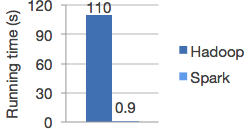
\includegraphics[width=0.5\textwidth]{../images/logistic-regressionSpark.png}
			\caption{Logistic Regression speedup on MLLib over haddop $^{[3]}$}
		\end{figure}
		\paragraph{CUDA}
		Having had experience with logistic regression and CUDA in the past, I coded my own solution to the problem. However, it is important to note that there are some solutions available from NVIDIA, include their NVIDIA Deep Learning SDK $^{[4]}$. I chose to code my own solution as to better understand and manipulate the execution of the logistic regression algorithm. I think it would be another interesting question to see how my implementation fairs to the solution provided by NVIDIA.
		
	\end{subsection}
\end{section}

\begin{section}{Results}
\paragraph{Spark}
Shown in figure 2 below, we have our results on the number of iterations of logistic regression possible in a ten minute window. The primary result is that with increasing number of worker nodes available, we do not see linear speed up, but rather a roughly 33\% speedup. This is roughly true for both 1 and 4 iterations of the algorithm, with an un-intuitive result on 2 maximum iterations. The second result to take from this is that increasing number of maximum iterations allow for better avg per iteration performance.
\begin{figure}[H]
	\centering
	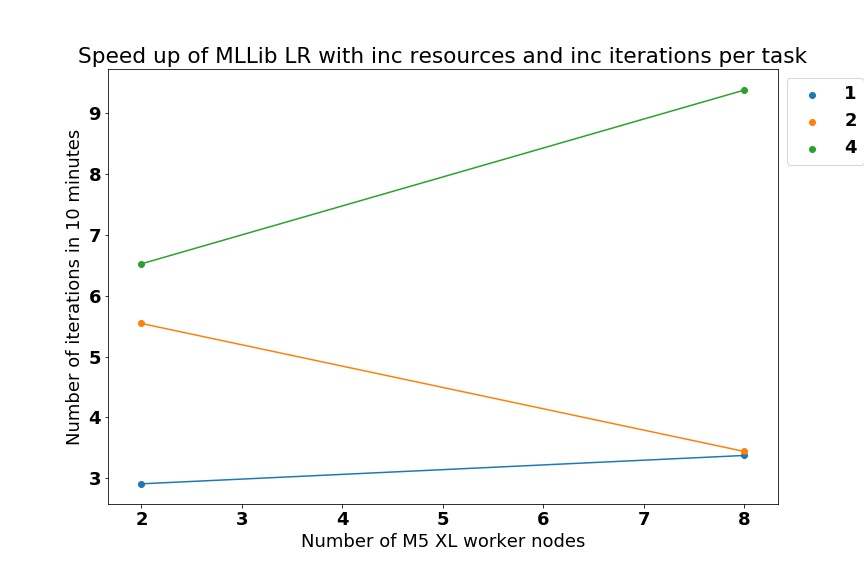
\includegraphics[width=0.8\textwidth]{../images/sparkResults.jpg}
	\caption{minimal speedup found over increasing core count. However iteration rate increases with increasing max iterations over the dataset}
\end{figure}

\paragraph{CUDA}
Shown in figure 3 below, we have our results of running logistic regression on our GTX 960 with increasing thread count on the $\log_2$ scale. The y-axis, similar to the previous results for Spark, show on average how many iterations of logistic regression can be calculated in a ten minute window.
\begin{figure}[H]
	\centering
	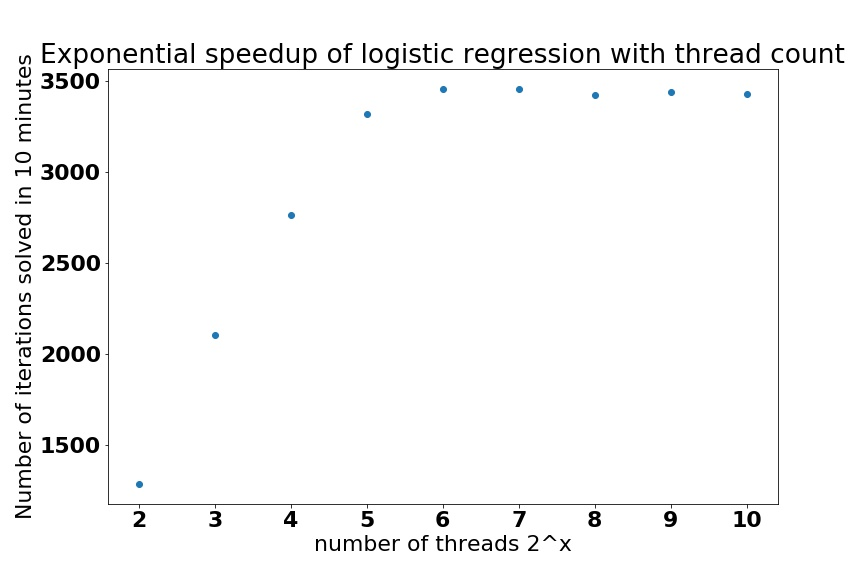
\includegraphics[width=0.8\textwidth]{../images/CUDAResults.jpg}
	\caption{less than linear speedup with doubling thread count on GTX 960 observed over logistic regression iterations in 10 minute windows}
\end{figure}

\end{section}

\begin{section}{Conclusion}
	Overall, the most clear sign of linear speedup was shown on the CUDA based logistic regression task. As we double the number of threads available to our computations, we seem to initially double the number of iterations possible in our ten minute window (1000$>$ to 2000$>$). However, this levels out  gradually until completely leveling out at about 32 threads. There are several potential reasons for this bottleneck.
	\paragraph{Locking} There is a contention on the lock to update the weights of our model. With every row of data, the graphics card needs to lock on each parameter of the model, to create the total loss. More details on this lock contention can be seen by viewing the kernel code available in the repository linked at the beginning of this paper.
	\paragraph{Iterative slowdown} Graphics cards are best for performing small arithmetic operations and then continuing on asynchronously to the next. This is possible due to their abundance of arithmetic logical units. However, they are slow(er) to handle long iterative processes compared to CPUs. $^{[5]}$
	\\
	\\
	For both of these reasons, I think we could see some bottle necking around the 32 threads. However, how do we explain Spark's performance?
	\\
	\\
	Spark was built to improve over its predecessor, MapReduce, to address various shortcomings the algorithm had on various application $^{[6]}$. One of its major advantages is that it maintains data in-memory and allows for constant iteration over the same data, rather than writing and reading it from disk $^{[6]}$. So how does this account for the drastic reduction in performance per-iteration compared to CUDA?
	
	\paragraph{Communication} Spark must distribute the data to all worker nodes. For logistic regression it likely sends subsets of data to each worker nodes, who computes its local iteration of logistic regression. At the end of its iteration, it likely has a communication round to make sure all nodes have the same weight updates for the coefficients. However, the largest cost comes from its first communication round moving data to the correct nodes. Afterwards, we can take advantage of the data being in-memory to compute another iteration of logistic regression much faster than map reduce. This heavy cost due to first round communication explains why we see a per-iteration boost in performance when we run more iterations on the data for both two and eight node. The exception being the performance of 2 iterations on 8 nodes. It could be that the cost of communication to all 8 worker nodes is still much higher that the benefit of only two iterations. 
	
	\paragraph{Data size} Spark is meant to handle very large datasets and long running operations, which is due to the use of Resilient Distributed Data Dataset(RDD) and lineage graphs for reliable computing $^{[5]}$. These in tandem with checkpointing allow Spark to handle large data and failures efficiently, especially compared to local machines. However, our data size is relatively small, only 0.5 GB. Consequently, it could be that for much larger data sizes, its ability to handle failures and fit large datasets in memory could provide much greater improvement on a per-iteration level compared to CUDA. However, this still needs to be tested.
	
	\begin{subsection}{Take-aways}
		\begin{itemize}
			\item CUDA has great linear speedup, limited by bottlenecks of iterative code and locking mechanisms
			\item Spark shows promising boosts in per iteration performance if given enough iterations to run, but has a heavy startup cost
			\item CUDA greatly outperforms Spark for smaller datasets and should be used accordingly with the principles of bottlenecks of CUDA kept in mind. Heavily iterative code may best be left for CPU intensive EMR clusters.
		\end{itemize}	
	\end{subsection}
	
\end{section}

\begin{section}{Future Work}
\paragraph{Better parallelism}
Both CUDA and Spark could be further optimized to boost computation speeds. For example, CUDA could take greater advantage of using more memory to store temporary values and avoid lock contention, or trying spin locks on high contention resources. Meanwhile, Spark may be able to use parallelism on the worker nodes if there are multiple threads available.
\paragraph{Scale up}
As aforementioned, this is a relatively small dataset for Spark to handle. If we increase our data by multiple factors, will CUDA be able to keep up if we cant fit it all in memory? Similarly, how well will Spark perform as we scale up our data?
\paragraph{More locks}
What if we need to lock more often than we have? What number of locking segments of code will cause Spark to outperform CUDA?
\paragraph{Combination}
It is trivial to see that we can likely use CUDA and Spark together to great success. How would this fare to using either on its own for various tasks?
\end{section}



\begin{section}{References}
\paragraph{[1]} (2019, Jan). GEFORCE GTX 900 SERIES GRAPHICS CARDS. Retrieved from https://www.nvidia.com/en-us/geforce/900-series/
\paragraph{[2]} Schofield, J. R., Carmichael, R., Tindemans, S., Bilton, M., Woolf, M., \& Strbac, G. (2015). Low Carbon London project: Data from the dynamic time-of-use electricity pricing trial, 2013. [data collection]. UK Data Service.
\paragraph{[3]} (2019, Jan), MLlib. Retrieved from https://spark.apache.org/mllib/
\paragraph{[4]} (2019, Jan), Deep Learning Frameworks. Retrieved from https://developer.nvidia.com/deep-learning-software
\paragraph{[5]} Omnisci, (2019, Jan), CPU to GPU. Retrieved from https://www.omnisci.com/learn/resources/technical-glossary/CPU-to-GPU
\paragraph{[6]} Zaharia, M., Chowdhury, M., Das, T., Dave, A., Ma, J., McCauley, M., ... \& Stoica, I. (2012, April). Resilient distributed datasets: A fault-tolerant abstraction for in-memory cluster computing. In Proceedings of the 9th USENIX conference on Networked Systems Design and Implementation (pp. 2-2). USENIX Association.
\end{section}
\\
\text{Have a great Holiday Season!}
\end{document}
